\documentclass[a4paper]{article}
\usepackage[mongolian]{babel}
\usepackage[utf8x]{inputenc}
\usepackage{listings, paralist}
\usepackage{xcolor}
\usepackage{graphicx}
\usepackage{float}
\usepackage{url}
\lstset{
    language=Python,
    basicstyle=\ttfamily,
    keywordstyle=\color{blue}\ttfamily,
    stringstyle=\color{red}\ttfamily,
    commentstyle=\color{green}\ttfamily,
    morecomment=[l][\color{magenta}]{\#},
    showspaces=false,   
    showstringspaces=false,
    extendedchars=true,
    breaklines=true,    
    breakatwhitespace=false,
    postbreak=\space,   
    tabsize=2,
    frame=single,       
    frameround=ffff,
    aboveskip=1.5em,
    literate={-}{-\allowbreak}1,
    numbers=left,
    stepnumber=1
}

\title{Хэв Танилтын Үндэс - Лаборатори 1}
\author{Э.Тэмүүжин,  20B1NUM1970}

\begin{document}
\maketitle

\section{Удиртгал}
Фолдероос зургууд уншаад дундаж зураг олж,  зураг нэг бүрийг дунджаас хасаад өөр фолдерт бичих.
\section{Хэрэгжүүлэлт}
Бид фолдероос зургуудыг олно. Үүний дараагаар олсон бүх зургуудыг уншиж, хэмжээг нь ижилхэн болгож эцэст саарал болгоно. Ингэснээр зураг бүрийн дунджийг олох боломжтой болно.

\subsection{Фолдероос зургууд уншихад бэлдэх}
\begin{lstlisting}
image_files = os.listdir(".")
image_files = [file for file in image_files if file.lower().endswith((".jpeg", ".jpg", ".png"))]
num_images = len(image_files)

avg_img = np.zeros((400, 500))
\end{lstlisting}

Эхний мөрөнд \textit{os.listdir(".")} ашиглан код байгаа фолдер доторх бүх файлуудын нэрийг авч байна.  Олсон файлын нэрсээс зурган файлыг \textit{2}-р мөрөнд авч байна. 

\subsection{Фолдер дах зургуудтай танилцах}
\begin{lstlisting}
fig, axs = plt.subplots(5, 2, figsize = (10, 15))

for ind, img_name in enumerate(image_files):
    img = cv2.imread(img_name)
    img = cv2.cvtColor(img, cv2.COLOR_BGR2RGB)
    img = cv2.resize(img, (500, 400))
    
    img_gray = cv2.cvtColor(img, cv2.COLOR_BGR2GRAY)
    avg_img = avg_img + img_gray/num_images

    axs[ind][0].imshow(img)
    axs[ind][0].set_title("RGB")

    axs[ind][1].imshow(img_gray, cmap = 'gray')
    axs[ind][1].set_title("Grayscale")

    axs[ind][0].set_axis_off()
    axs[ind][1].set_axis_off()
\end{lstlisting}

\begin{itemize}
\item \textit{4}-р мөр: Зураг уншиж байна
\item \textit{5}-р мөр: \textit{Open-CV} сан нь зургийг BGR дарааллаар уншдаг тул уншсан зургийн өнгөний сувгийн дарааллыг RGB болгоно
\item \textit{6}-р мөр: Зургийн хэмжээг өөрчилж байна
\item \textit{8}-р мөр: Өнгөт зургийг саарал болгоно
\item \textit{9}-р мөр: Зургийн дунджийг олох
\end{itemize}


\subsection{Зураг бүрийг дунджаас хасах}
\begin{lstlisting}
fig, axs = plt.subplots(5, 2, figsize = (10, 15))

for ind, img_name in enumerate(image_files):
    img = cv2.imread(img_name)
    img = cv2.cvtColor(img, cv2.COLOR_BGR2GRAY)
    img = cv2.resize(img, (500, 400))
    
    img_sub = avg_img - img

    axs[ind][0].imshow(img, cmap = 'gray')
    axs[ind][0].set_title("Before")

    axs[ind][1].imshow(img_sub, cmap = 'gray')
    axs[ind][1].set_title("After")

    axs[ind][0].set_axis_off()
    axs[ind][1].set_axis_off()

    cv2.imwrite(f"./Result/{img_name}_sub.jpg", img_sub)
\end{lstlisting}
Энд \textit{8}-р мөрөнд дундажаас зураг хасаж байна.  Үүссэн зургийг \textit{19}-р мөрөнд \textbf{Result} фолдерт хадгална.

\section{Үр дүн}
\subsection{Фолдер дах зургуудтай танилцах}
\begin{figure}[H]
  \centering
  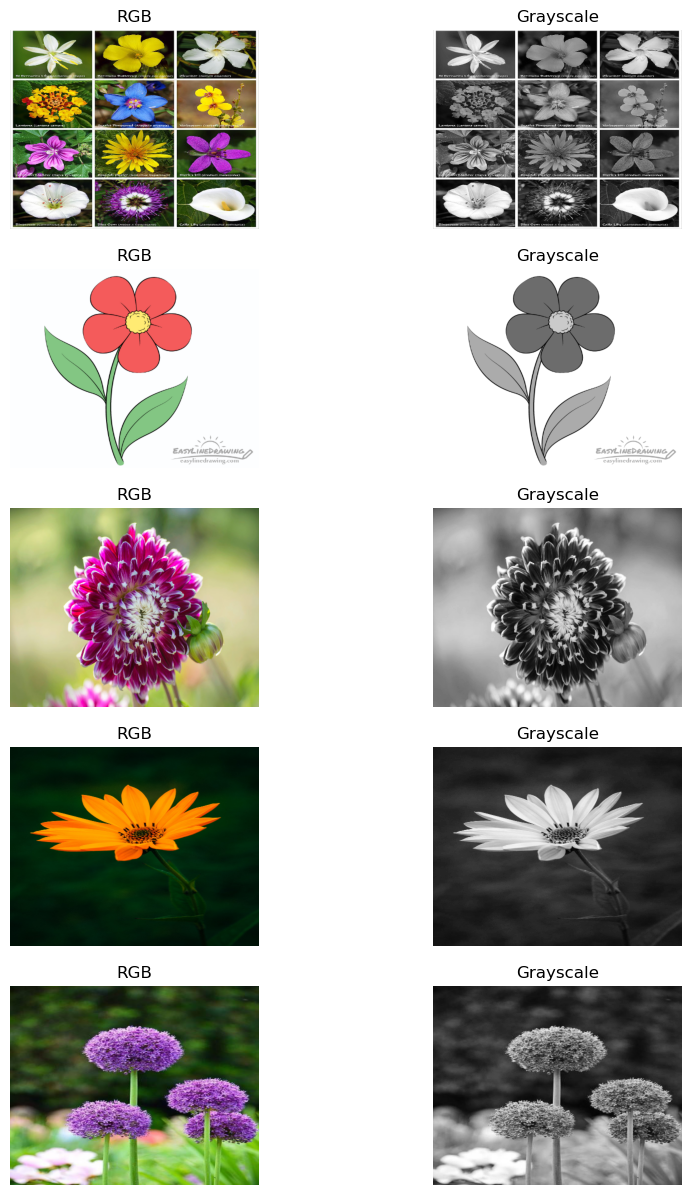
\includegraphics[scale = 0.5]{img1.png}
  \caption[Caption for Pointer example]{Анхны зургууд}
  \label{fig:example_1}
\end{figure}

\subsection{Зураг бүрийг дунджаас хасах}
Энд зүүн баганад (\textit{Before}) анхны зургийг үзүүлж байгаа ба баруун талд (\textit{After}) уг зургийг нийт зургийн дунджаас хасахад үүссэн зургийг үзүүлж байна.
\begin{figure}[H]
  \centering
  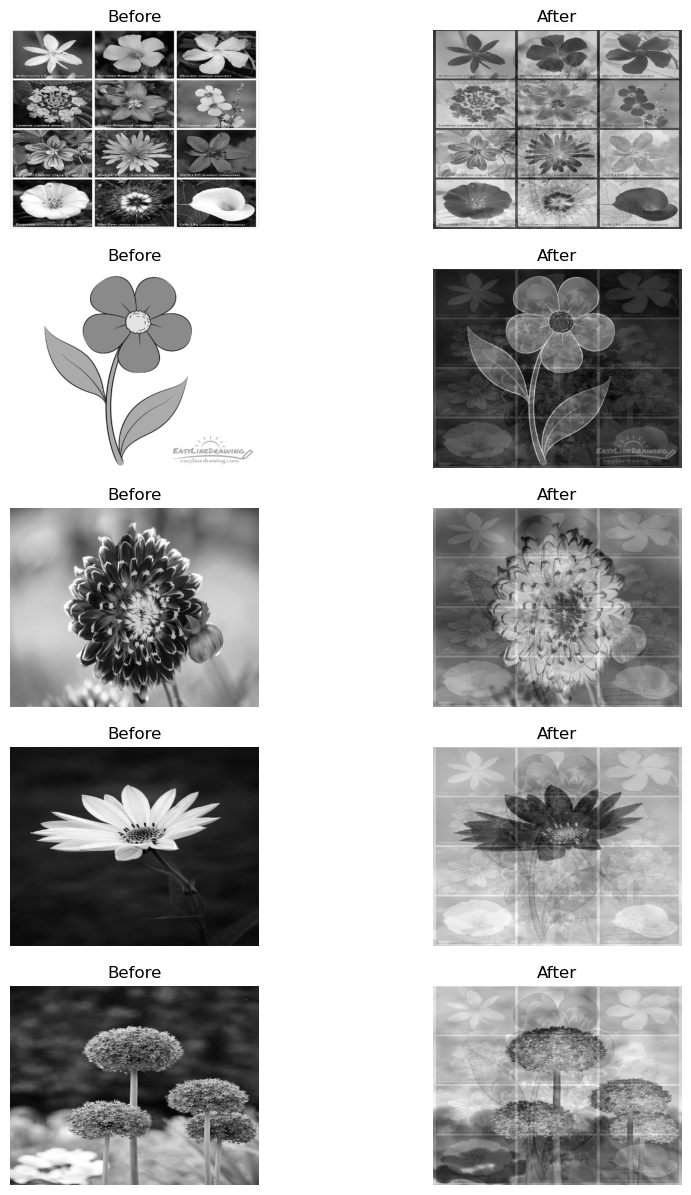
\includegraphics[scale = 0.5]{img2.png}
  \caption[Caption for Pointer example]{Зураг бүрээс хассан нийт зургуудын дунджийг хассан зургууд}
  \label{fig:example_1}
\end{figure}



\end{document}